% Subgroup lattices of D4 (left) and Z/12 (right); normal subgroups in blue boxes. Generated by a short script.
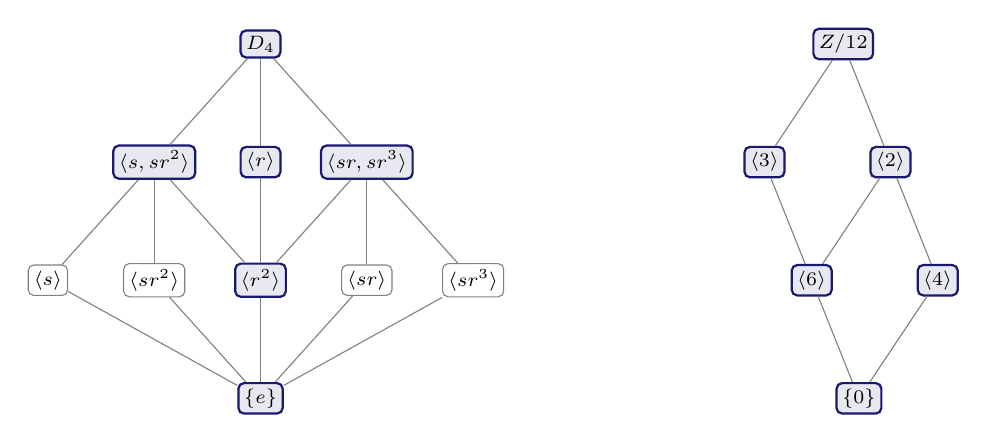
\begin{tikzpicture}[sub/.style={font=\scriptsize,inner sep=2pt,rounded corners=2pt},nor/.style={sub,draw=MidnightBlue,fill=MidnightBlue!10,thick},oth/.style={sub,draw=gray}]
\node[nor] (d0) at (0.00,0.00) {$\{e\}$};
\node[nor] (d1) at (0.00,1.50) {$\langle r^2\rangle$};
\node[oth] (d2) at (-2.70,1.50) {$\langle s\rangle$};
\node[oth] (d3) at (1.35,1.50) {$\langle sr\rangle$};
\node[oth] (d4) at (-1.35,1.50) {$\langle sr^2\rangle$};
\node[oth] (d5) at (2.70,1.50) {$\langle sr^3\rangle$};
\node[nor] (d6) at (0.00,3.00) {$\langle r\rangle$};
\node[nor] (d7) at (-1.35,3.00) {$\langle s,sr^2\rangle$};
\node[nor] (d8) at (1.35,3.00) {$\langle sr,sr^3\rangle$};
\node[nor] (d9) at (0.00,4.50) {$D_4$};
\draw[gray] (d3) -- (d8);
\draw[gray] (d5) -- (d8);
\draw[gray] (d0) -- (d3);
\draw[gray] (d0) -- (d5);
\draw[gray] (d0) -- (d2);
\draw[gray] (d0) -- (d4);
\draw[gray] (d0) -- (d1);
\draw[gray] (d2) -- (d7);
\draw[gray] (d4) -- (d7);
\draw[gray] (d7) -- (d9);
\draw[gray] (d1) -- (d7);
\draw[gray] (d1) -- (d6);
\draw[gray] (d1) -- (d8);
\draw[gray] (d6) -- (d9);
\draw[gray] (d8) -- (d9);
\node[nor] (z1) at (7.60,0.00) {$\{0\}$};
\node[nor] (z2) at (7.00,1.50) {$\langle 6\rangle$};
\node[nor] (z3) at (8.60,1.50) {$\langle 4\rangle$};
\node[nor] (z4) at (6.40,3.00) {$\langle 3\rangle$};
\node[nor] (z6) at (8.00,3.00) {$\langle 2\rangle$};
\node[nor] (z12) at (7.40,4.50) {$\mathbb Z/12$};
\draw[gray] (z1) -- (z2);
\draw[gray] (z1) -- (z3);
\draw[gray] (z2) -- (z4);
\draw[gray] (z2) -- (z6);
\draw[gray] (z3) -- (z6);
\draw[gray] (z4) -- (z12);
\draw[gray] (z6) -- (z12);
\end{tikzpicture}
